% Options for packages loaded elsewhere
\PassOptionsToPackage{unicode}{hyperref}
\PassOptionsToPackage{hyphens}{url}
\PassOptionsToPackage{dvipsnames,svgnames*,x11names*}{xcolor}
%
\documentclass[
  8pt,
  ignorenonframetext,
  dvipsnames]{beamer}
\usepackage{pgfpages}
\setbeamertemplate{caption}[numbered]
\setbeamertemplate{caption label separator}{: }
\setbeamercolor{caption name}{fg=normal text.fg}
\beamertemplatenavigationsymbolsempty
% Prevent slide breaks in the middle of a paragraph
\widowpenalties 1 10000
\raggedbottom
\setbeamertemplate{part page}{
  \centering
  \begin{beamercolorbox}[sep=16pt,center]{part title}
    \usebeamerfont{part title}\insertpart\par
  \end{beamercolorbox}
}
\setbeamertemplate{section page}{
  \centering
  \begin{beamercolorbox}[sep=12pt,center]{part title}
    \usebeamerfont{section title}\insertsection\par
  \end{beamercolorbox}
}
\setbeamertemplate{subsection page}{
  \centering
  \begin{beamercolorbox}[sep=8pt,center]{part title}
    \usebeamerfont{subsection title}\insertsubsection\par
  \end{beamercolorbox}
}
\AtBeginPart{
  \frame{\partpage}
}
\AtBeginSection{
  \ifbibliography
  \else
    \frame{\sectionpage}
  \fi
}
\AtBeginSubsection{
  \frame{\subsectionpage}
}
\usepackage{lmodern}
\usepackage{amssymb,amsmath}
\usepackage{ifxetex,ifluatex}
\ifnum 0\ifxetex 1\fi\ifluatex 1\fi=0 % if pdftex
  \usepackage[T1]{fontenc}
  \usepackage[utf8]{inputenc}
  \usepackage{textcomp} % provide euro and other symbols
\else % if luatex or xetex
  \usepackage{unicode-math}
  \defaultfontfeatures{Scale=MatchLowercase}
  \defaultfontfeatures[\rmfamily]{Ligatures=TeX,Scale=1}
\fi
% Use upquote if available, for straight quotes in verbatim environments
\IfFileExists{upquote.sty}{\usepackage{upquote}}{}
\IfFileExists{microtype.sty}{% use microtype if available
  \usepackage[]{microtype}
  \UseMicrotypeSet[protrusion]{basicmath} % disable protrusion for tt fonts
}{}
\makeatletter
\@ifundefined{KOMAClassName}{% if non-KOMA class
  \IfFileExists{parskip.sty}{%
    \usepackage{parskip}
  }{% else
    \setlength{\parindent}{0pt}
    \setlength{\parskip}{6pt plus 2pt minus 1pt}}
}{% if KOMA class
  \KOMAoptions{parskip=half}}
\makeatother
\usepackage{xcolor}
\IfFileExists{xurl.sty}{\usepackage{xurl}}{} % add URL line breaks if available
\IfFileExists{bookmark.sty}{\usepackage{bookmark}}{\usepackage{hyperref}}
\hypersetup{
  pdftitle={Introduction to Multivariate Regression \& Econometrics},
  pdfauthor={Lecture 2},
  colorlinks=true,
  linkcolor=Maroon,
  filecolor=Maroon,
  citecolor=Blue,
  urlcolor=blue,
  pdfcreator={LaTeX via pandoc}}
\urlstyle{same} % disable monospaced font for URLs
\newif\ifbibliography
\usepackage{graphicx,grffile}
\makeatletter
\def\maxwidth{\ifdim\Gin@nat@width>\linewidth\linewidth\else\Gin@nat@width\fi}
\def\maxheight{\ifdim\Gin@nat@height>\textheight\textheight\else\Gin@nat@height\fi}
\makeatother
% Scale images if necessary, so that they will not overflow the page
% margins by default, and it is still possible to overwrite the defaults
% using explicit options in \includegraphics[width, height, ...]{}
\setkeys{Gin}{width=\maxwidth,height=\maxheight,keepaspectratio}
% Set default figure placement to htbp
\makeatletter
\def\fps@figure{htbp}
\makeatother
\setlength{\emergencystretch}{3em} % prevent overfull lines
\providecommand{\tightlist}{%
  \setlength{\itemsep}{0pt}\setlength{\parskip}{0pt}}
\setcounter{secnumdepth}{-\maxdimen} % remove section numbering

%packages
\usepackage{graphicx}
\usepackage{rotating}
\usepackage{hyperref}

\usepackage{tikz} % used for text highlighting, amongst others
\usepackage{comment}

%title slide stuff
%\institute{Department of Education}
%\title{Managing and Manipulating Data Using R}

%
\setbeamertemplate{navigation symbols}{} % get rid of navigation icons:
\setbeamertemplate{footline}[page number]

%\setbeamertemplate{frametitle}{\thesection \hspace{0.2cm} \insertframetitle}
\setbeamertemplate{section in toc}[sections numbered]
%\setbeamertemplate{subsection in toc}[subsections numbered]
\setbeamertemplate{subsection in toc}{%
  \leavevmode\leftskip=3.2em\color{gray}\rlap{\hskip-2em\inserttocsectionnumber.\inserttocsubsectionnumber}\inserttocsubsection\par
}

%define colors
%\definecolor{uva_orange}{RGB}{216,141,42} % UVa orange (Rotunda orange)
\definecolor{mygray}{rgb}{0.95, 0.95, 0.95} % for highlighted text
	% grey is equal parts red, green, blue. higher values >> lighter grey
	%\definecolor{lightgraybo}{rgb}{0.83, 0.83, 0.83}

% new commands

%highlight text with very light grey
\newcommand*{\hlg}[1]{%
	\tikz[baseline=(X.base)] \node[rectangle, fill=mygray] (X) {#1};%
}
%, inner sep=0.3mm
%highlight text with very light grey and use font associated with code
\newcommand*{\hlgc}[1]{\texttt{\hlg{#1}}}

%modifying back ticks to add grey background
\let\OldTexttt\texttt
\renewcommand{\texttt}[1]{\OldTexttt{\hlg{#1}}}


\begin{comment}

% Font
\usepackage[defaultfam,light,tabular,lining]{montserrat}
\usepackage[T1]{fontenc}
\renewcommand*\oldstylenums[1]{{\fontfamily{Montserrat-TOsF}\selectfont #1}}

% Change color of boldface text to darkgray
\renewcommand{\textbf}[1]{{\color{darkgray}\bfseries\fontfamily{Montserrat-TOsF}#1}}

% Bullet points
\setbeamertemplate{itemize item}{\color{BlueViolet}$\circ$}
\setbeamertemplate{itemize subitem}{\color{BrickRed}$\triangleright$}
\setbeamertemplate{itemize subsubitem}{$-$}

% Reduce space before lists
%\addtobeamertemplate{itemize/enumerate body begin}{}{\vspace*{-8pt}}

\let\olditem\item
\renewcommand{\item}{%
  \olditem\vspace{4pt}
}

% decreasing space before and after level-2 bullet block
%\addtobeamertemplate{itemize/enumerate subbody begin}{}{\vspace*{-3pt}}
%\addtobeamertemplate{itemize/enumerate subbody end}{}{\vspace*{-3pt}}

% decreasing space before and after level-3 bullet block
%\addtobeamertemplate{itemize/enumerate subsubbody begin}{}{\vspace*{-2pt}}
%\addtobeamertemplate{itemize/enumerate subsubbody end}{}{\vspace*{-2pt}}

%Section numbering
\setbeamertemplate{section page}{%
    \begingroup
        \begin{beamercolorbox}[sep=10pt,center,rounded=true,shadow=true]{section title}
        \usebeamerfont{section title}\thesection~\insertsection\par
        \end{beamercolorbox}
    \endgroup
}

\setbeamertemplate{subsection page}{%
    \begingroup
        \begin{beamercolorbox}[sep=6pt,center,rounded=true,shadow=true]{subsection title}
        \usebeamerfont{subsection title}\thesection.\thesubsection~\insertsubsection\par
        \end{beamercolorbox}
    \endgroup
}

\end{comment}

\title{Introduction to Multivariate Regression \& Econometrics}
\subtitle{HED 612}
\author{Lecture 2}
\date{}

\begin{document}
\frame{\titlepage}

\begin{frame}
  \tableofcontents[hideallsubsections]
\end{frame}
\hypertarget{prep}{%
\section{Prep}\label{prep}}

\begin{frame}{Download Data and Open R Script}
\protect\hypertarget{download-data-and-open-r-script}{}

\emph{If you had trouble installing R/ R Studio, let me know before
moving forward}

\medskip

\emph{Download Data and Open R Script}

\begin{enumerate}
\tightlist
\item
  Create a new data folder called ``ca''

  \begin{itemize}
  \tightlist
  \item
    hed612 \textgreater\textgreater\textgreater{} data
    \textgreater\textgreater\textgreater{} ca
  \end{itemize}
\item
  Download the California Dataset from D2L (under Data)

  \begin{itemize}
  \tightlist
  \item
    Place the ``caschool-v2.dta'' dataset into the ``ca'' folder you
    created in the previous step
  \end{itemize}
\item
  Download the Lecture 2 PDF and R script for this week

  \begin{itemize}
  \tightlist
  \item
    Place all files in hed612 \textgreater\textgreater\textgreater{}
    lectures \textgreater\textgreater\textgreater{} lecture2
  \end{itemize}
\item
  Open the RProject you created last week (should be in your main
  HED612\_S21 folder)
\item
  Once the RStudio window opens, open the Lecture 2 R script by clicking
  on:

  \begin{itemize}
  \tightlist
  \item
    file \textgreater\textgreater\textgreater{} open file\ldots{}
    \textgreater\textgreater\textgreater{} {[}navigate to lecture 2
    folder{]} \textgreater\textgreater\textgreater{} lecture2.R
  \end{itemize}
\end{enumerate}

\end{frame}

\begin{frame}{Review Homework}
\protect\hypertarget{review-homework}{}

\begin{itemize}
\tightlist
\item
  Every week we will spend 10-15 min s a class or in groups reviewing
  the problem set you just submitted
\item
  Problem Set \#1 Common Questions {[}review as a class{]}

  \begin{itemize}
  \tightlist
  \item
    Why same Q4 and Q5?

    \begin{itemize}
    \tightlist
    \item
      I will often ask same questions multiple times seeking different
      solutions
    \item
      Absolute and relative filepaths will techinically get you to the
      ``right'' answer; I want you to understand/get practice with the
      difference between these two approaches
    \end{itemize}
  \item
    Why a word document and an R script?

    \begin{itemize}
    \tightlist
    \item
      Problem sets will ask both ``substantive'' questions and ``R
      syntax/code'' questions
    \item
      R scripts should only contain R syntax/code and short comments
      describing what you are doing via the R syntax/code
    \item
      Word documents should be used for substantive answers; no need to
      copy in R syntax/code into the word document
    \end{itemize}
  \end{itemize}
\item
  Questions or Concerns?
\item
  Solutions to all problem sets with be posted on D2L after I finish
  grading
\item
  If you need a bit more help with absolute/relative file paths

  \begin{itemize}
  \tightlist
  \item
    YouTube Video:
    \url{https://www.youtube.com/watch?v=ephId3mYu9o\&t=1s}
  \end{itemize}
\end{itemize}

\end{frame}

\begin{frame}{Today and Next Week}
\protect\hypertarget{today-and-next-week}{}

\textbf{Today}

\begin{itemize}
\tightlist
\item
  Review of statistics {[}univariate{]}
\item
  R Basics
\end{itemize}

\medskip

\textbf{HW \& Reading}

\begin{itemize}
\tightlist
\item
  HW\#2 posted on D2L
\item
  No reading for next week
\end{itemize}

\medskip

\textbf{Next Week}

\begin{itemize}
\tightlist
\item
  Review of Statistics {[}bivariate{]}
\item
  Introduction to bivariate regression
\end{itemize}

\end{frame}

\hypertarget{review-of-statistics}{%
\section{Review of Statistics}\label{review-of-statistics}}

\begin{frame}{Statistical Inference}
\protect\hypertarget{statistical-inference}{}

\emph{Goal of statistical inference is to infer something about the
population from a sample}

\medskip

\textbf{Population Parameter}: a measure of the population

\begin{itemize}
\tightlist
\item
  e.g., mean household income for all U.S. households; proportion of all
  American voters approving president's performance;
\item
  We don't know this 99.9999999\% of the time because we don't have data
  on the entire population
\end{itemize}

\medskip

\textbf{Sample} is part of, a subset, of the population

\medskip

\textbf{Estimator (or Statistic)}: a formula or procedure used to
estimate the value of the population parameter using a sample of the
population

\begin{itemize}
\tightlist
\item
  e.g., formula to calculate sample mean (\(\bar{Y}\)) or sample
  proportion (\(\hat{p}\))
\end{itemize}

\medskip

\textbf{Point Estimate}: numeric value generated from calculating an
estimator from a specific sample of data

\begin{itemize}
\tightlist
\item
  e.g., sample mean household income is \$81,000, 2017 American
  Community Survey
\end{itemize}

\end{frame}

\begin{frame}{Parameters and Point Estimates}
\protect\hypertarget{parameters-and-point-estimates}{}

Introductory statistics class

\begin{itemize}
\tightlist
\item
  Parameter: Population mean (\(\mu_Y\))
\item
  Estimator: Sample mean (\(\bar{Y}\))
\item
  RQs: What is the mean GPA of UA students living in residence halls?
\end{itemize}

\medskip

Multivariate regression class

\begin{itemize}
\tightlist
\item
  Parameter: Population regression coefficient (\(\beta\))
\item
  Estimator: Sample regression coefficient (\(\hat{\beta}\))
\item
  RQs: What is the effect of living in residence halls on GPA?
\end{itemize}

\end{frame}

\begin{frame}{Notation for Parameters}
\protect\hypertarget{notation-for-parameters}{}

Population Parameters

\begin{itemize}
\tightlist
\item
  Denoted by Greek setters, usually lowercase

  \begin{itemize}
  \tightlist
  \item
    \(\mu\) : ``mu'' refers to population mean
  \item
    \(\sigma\): ``sigma'' refers to population standard deviation
  \item
    \(\beta\): ``beta'' refers to population regression coefficient
  \end{itemize}
\item
  Subscripts usually denote population parameters of certain variables

  \begin{itemize}
  \tightlist
  \item
    \(\mu_Y\) : ``mu Y'' refers to population mean of the variable Y
  \item
    \(\sigma_X\): ``sigma X'' refers to population standard deviation of
    the variable X
  \end{itemize}
\end{itemize}

\medskip

Estimators of Population Parameters (two general approaches)

\begin{itemize}
\tightlist
\item
  Denoted using Greek letters with a ``hat''

  \begin{itemize}
  \tightlist
  \item
    \(\hat{\mu}_Y\) : ``mu Y hat'' refers to the estimate of \(\mu_Y\)
  \item
    \(\hat{\beta}_X\): ``beta X hat'' refers to the estimate of
    \(\beta_X\)
  \end{itemize}
\item
  Denoted using English/Arabic letters

  \begin{itemize}
  \tightlist
  \item
    \(\bar{Y}\): ``Y bar'' refers to the estimate of \(\mu_Y\)
  \item
    \(s_X\): ``S of X'' refers to the estimate of \(\sigma_X\)
  \end{itemize}
\end{itemize}

\end{frame}

\begin{frame}{Data Sources}
\protect\hypertarget{data-sources}{}

\textbf{Experimental Data}: obtained from experiments designed to assess
the causal effect of a ``treatment'' on an outcome

\begin{itemize}
\tightlist
\item
  randomized control trials (experiments) are the \textbf{gold standard}
  of program evaluation {[}will learn more about this{]}
\item
  e.g., Tennessee STAR project
\end{itemize}

\medskip
\medskip

\textbf{Observational Data}: obtained from surveys, administrative
records {[}focus of this course{]}

\begin{itemize}
\tightlist
\item
  researchers have/had no control on the ``treatment''
\item
  e.g., Beginning Postsecondary Students Longitudinal Study, High School
  Longitudinal Study, National Education Longitudinal Study
\end{itemize}

\end{frame}

\begin{frame}{Data Types}
\protect\hypertarget{data-types}{}

\textbf{Cross sectional data}: data on different ``observations'' (e.g.,
students, classrooms, universities) for a single point in time {[}focus
of this course{]}

\begin{itemize}
\tightlist
\item
  e.g., California Test Score data where ``observations'' are districts
\end{itemize}

\medskip

\textbf{Time-Series Data}: data on a single ``observation'' collected at
multiple time points

\begin{itemize}
\tightlist
\item
  e.g., US inflation and unemployment rate data 1959-2000
\end{itemize}

\medskip

\textbf{Longitudinal Data} (or panel data): data on multiple
``observations'' at multiple time points

\begin{itemize}
\tightlist
\item
  e.g., Beginning Postsecondary Students Longitudinal Study, High School
  Longitudinal Study, National Education Longitudinal Study
\end{itemize}

\end{frame}

\begin{frame}{Variables}
\protect\hypertarget{variables}{}

\textbf{Continuous Variables}

\begin{itemize}
\tightlist
\item
  Variables that take on a continuum of possible values where the
  distance between one value and another is meaningful
\item
  Examples: Age, income, GPA, test scores
\end{itemize}

\medskip

\textbf{Discrete Variables} (or categorical variables)

\begin{itemize}
\tightlist
\item
  Variables that can only take on specific (discrete) integer values
\item
  Can be nominal (school type), ordinal (likert scale), and quantitative
  (number of children)
\end{itemize}

\end{frame}

\begin{frame}{Measures of Central Tendency: Sample Mean}
\protect\hypertarget{measures-of-central-tendency-sample-mean}{}

Sample mean of Y or denoted as \(\bar{Y}\)

\begin{itemize}
\tightlist
\item
  \(\bar{Y} = \frac{\sum_{i=1}^{n} Y_i}{n}\)

  \begin{itemize}
  \tightlist
  \item
    where subscript \emph{i} refers to the observation i
  \end{itemize}
\end{itemize}

\medskip

Example: Variable Y has the following six observations (\(Y_1... Y_6\))

\begin{itemize}
\tightlist
\item
  Obs: \(Y_1 = 5, Y_1 = 2, Y_3 = 13, Y_4 = 11, Y_5 = 18, Y_6 = 22\)
\item
  Calculate \(\bar{Y}\)
\end{itemize}

\medskip

Other measures of central tendency:

\begin{itemize}
\tightlist
\item
  Median
\item
  Mode
\end{itemize}

\end{frame}

\begin{frame}{Measures of Dispersion: Standard Deviation}
\protect\hypertarget{measures-of-dispersion-standard-deviation}{}

Sample standard deviation of Y or denoted as \(\hat\sigma_Y\)

\begin{itemize}
\item
  Standard deviation is, on average, how far away a random observation,
  \(Y_i\), is from the sample mean, \(\bar{Y}\)
\item
  \(\hat\sigma_Y = \sqrt{\frac{\sum_{i=1}^N (Y_i - \overline{Y})^2}{N-1}}\)

  \begin{itemize}
  \tightlist
  \item
    ``square root of sum of squared deviations divided by n-1''
  \end{itemize}
\end{itemize}

\medskip

Example: Variable Y has the following six observations (\(Y_1... Y_6\))

\begin{itemize}
\tightlist
\item
  Obs: \(Y_1 = 5, Y_1 = 2, Y_3 = 13, Y_4 = 11, Y_5 = 18, Y_6 = 22\)
\item
  Calculate \(\hat\sigma_Y\)
\end{itemize}

\medskip

Other measures of dispersion:

\begin{itemize}
\tightlist
\item
  Variance (SD is the square root of the variance)
\item
  Range
\end{itemize}

\end{frame}

\begin{frame}{Sample Mean \& Standard Deviation}
\protect\hypertarget{sample-mean-standard-deviation}{}

Substantive interpretation(s):

\begin{itemize}
\tightlist
\item
  Which distribution has the greatest mean and lowest mean?
\item
  Which distribution has the greatest standard deviation and lowest
  standard deviation?
\end{itemize}

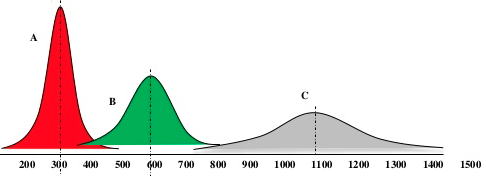
\includegraphics{distributions.png}

\end{frame}

\begin{frame}{Sample Mean \& Standard Deviation}
\protect\hypertarget{sample-mean-standard-deviation-1}{}

Substantive interpretation(s):

Consider the SAT scores of students at a large, public high school and
the SAT scores of the Harvard freshman class:

\begin{itemize}
\item
  Which do you think has a larger mean?
\item
  Which do you think has a larger standard deviation?
\end{itemize}

\end{frame}

\begin{frame}{Sampling Distribution \& Central Limit Theorem}
\protect\hypertarget{sampling-distribution-central-limit-theorem}{}

Many of the statistical tests we use (e.g., t-tests, confidence
intervals) assume that populations we work with are normally
distributed.

\begin{itemize}
\tightlist
\item
  A bit unrealistic (outliers, skewness, bimodal)
\end{itemize}

\medskip

An appropriate sample size and \emph{Central Limit Theorem} can help us
get around this assumption!

\begin{itemize}
\tightlist
\item
  We usually determine appropriate sample size via exploratory data
  analysis
\end{itemize}

\medskip

\textbf{Central Limit Theorem}: No matter the distribution of our
population parameter, given a suffficiently large sample size, the
sampling distribution of the estimate (e.g., mean) for a variable will
approximate a normal distribution.

\end{frame}

\begin{frame}{Sampling Distribution \& Central Limit Theorem}
\protect\hypertarget{sampling-distribution-central-limit-theorem-1}{}

Sampling Distribution

\begin{itemize}
\tightlist
\item
  \textbf{Mean of Sample Means} (\(\bar{Y}_Y\)) = population mean
  (\(\mu_Y\))
\item
  \textbf{Standard Error} \(SE(\bar{Y})\): the standard deviation of the
  sampling distribution. In other words it is the average distance
  between a random sample mean and the mean of sample means.
\end{itemize}

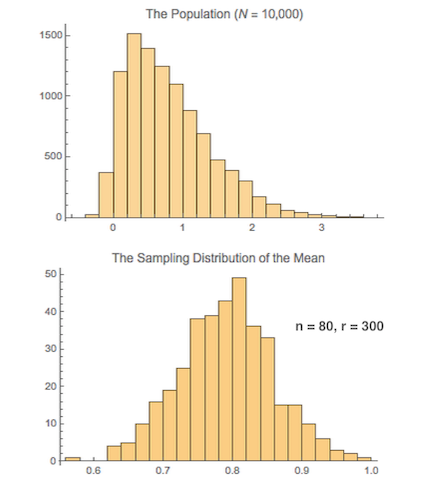
\includegraphics[width=150pt]{sampdist.png}

Interactive presentation
\href{http://onlinestatbook.com/stat_sim/sampling_dist/}{link}

\end{frame}

\hypertarget{min-break}{%
\section{10 Min Break}\label{min-break}}

\hypertarget{r-basics}{%
\section{R Basics}\label{r-basics}}

\begin{frame}[fragile]{R Script Basics}
\protect\hypertarget{r-script-basics}{}

Go to the lecture2.R script I had you download before class

\medskip

\textbf{Within an R script you can run commands in different ways}:

\begin{enumerate}
\tightlist
\item
  One command at a time by highlighting only that command and clicking
  the ``Run'' Button
\item
  Several commands at a time by highlighting several commands and
  clicking the ``Run'' Button
\item
  Run the entire R script by not highlighting any commands and clicking
  the ``Run'' Button
\end{enumerate}

\medskip

\textbf{Comments}

\begin{itemize}
\tightlist
\item
  \texttt{\#} Will comment out the remainder of syntax on that line
\item
  \texttt{"\ "} Will comment out anything between the quotation marks
  (multiple lines)
\end{itemize}

\end{frame}

\begin{frame}{Tidyverse}
\protect\hypertarget{tidyverse}{}

\begin{itemize}
\tightlist
\item
  R sytanx for this class will all be given to you.
\item
  For problem sets, you often will get an example of the code you need
  to run in the lecture or directly in the instructions; you'll often
  use that code as template for you the specific task you are working on
\item
  While you have the template; you will often need to change a ``couple
  of minor things'' (e.g., the variable name; the ``function'' for the
  statistical test you are trying to run, etc.)
\item
  So you will still need to develop some ``intuition'' as to what the
  code is doing
\item
  All code (very few exceptions) will be written in the ``tidyverse''
  way as opposed to base R

  \begin{itemize}
  \tightlist
  \item
    Base R: the ``default'' coding approach to R; it can be very
    inefficient
  \item
    Tidyverse: most popular way to write R code that does simple tasks
    (everything we do in this class is considered simple)
  \end{itemize}
\end{itemize}

\end{frame}

\begin{frame}[fragile]{Tidyverse}
\protect\hypertarget{tidyverse-1}{}

\begin{itemize}
\tightlist
\item
  Most distinctive part of Tidyverse approach to R syntax is using pipes
  or piping operator \texttt{\%\textgreater{}\%}

  \begin{itemize}
  \tightlist
  \item
    Allows for ``sequential computations'' or multiple commands/tasks in
    the same line of code
  \item
    I usually think of the words ``AND THEN'' every time I see a pipe
  \end{itemize}
\item
  \texttt{caschool\ \%\textgreater{}\%\ select(enrl\_tot,\ computer,\ read\_scr)\ \%\textgreater{}\%\ var\_label()}

  \begin{itemize}
  \tightlist
  \item
    \texttt{caschool}= open the california school dataset \textbf{AND
    THEN}
  \item
    \texttt{select(enrl\_tot,\ computer,\ read\_scr)} = select the three
    variables enrol\_tot, computer, read\_scr \textbf{AND THEN}
  \item
    \texttt{var\_label()} = print the labels for the three variables
    selected
  \end{itemize}
\end{itemize}

\end{frame}

\end{document}
